\documentclass[a4paper,12pt]{article}

% Packages
\usepackage[utf8]{inputenc}
\usepackage{amsmath}
\usepackage{graphicx}
\usepackage{hyperref}
\usepackage{geometry}

\usepackage{colortbl} % For coloring table cells and lines
\usepackage[table]{xcolor} % For more color options
\usepackage{booktabs}



\geometry{a4paper, margin=1in}

% Title and Author
\title{Exercise 1}
\author{Your Name}

\begin{document}

% Title Page
\maketitle

% Abstract
\begin{abstract}
This is the abstract of the document. It provides a brief summary of the content.
\end{abstract}

% Table of Contents
\tableofcontents
\newpage

% Sections
\section{Introduction}
This is the introduction section. Here you can introduce the topic of your document.

\section{Methodology}
This section describes the methodology used in your work.

\subsection{Subsection Example}
This is an example of a subsection.

\section{Preprocessing}
\label{sec:preprocessing}
We will do four different measures to properly preprocess the data. These are: data imputation, encoding of categorical variables,
scaling of numerical values and dimensionality reduction. In this section we will look at each dataset and 
describe which tasks can be used on the dataset and how a specific task is performed. Then we will compare the different
settings for all the models and determine their effectiveness using measures described in the previous section. 
In order to make this a meaningful comparison, we will use the default hyperparameters for all classifiers and 
we will split the data equally in the cross-validation.\\
Data leakage occurs when data is preprocessed before it was split into the training and test set. This way information 
from the test set is used to preprocess the training set. For example the MinMaxScaler uses the minimun and maximum values 
to scale these values properly. The values should only be computed on the training set and then be used on both training and 
test set. This can get rather difficult when using cross-validation. In order to avoid this, we will use the pipelines.    
Pipelines are a feature of scikit-learn that allow for the chaining of multiple transformers and estimators and also avoid 
data leakage. We will define a different pipeline for each preprocessing task and variant and chain these pipelines to compare 
the different settings.\\
\textbf{Congressional Voting:} As this dataset contains missing values we will need a strategy to impute these values. 
It is important to note that the missing values are all labeled as \textit{'unknown'}.
As all the values are categorical there are two possible strategies for data imputation.
We can either use the most frequent value of the respective attribute in the training dataset
or we can treat the missing values as a separate category. We will use one-hot-encoding for the categorical values,
except for the binary ones. Binary values will be encoded as 0 and 1. By using one-hot-encoding
the tow different treatments of the missing values will yield a different encoding. Still all the values remain binary, 
so no further scaling is needed. As the dataset is rather small, we will not use dimensionality reduction. This means
that we will only compare the two different strategies for data imputation.
In table~\ref{table:imputation} the results are visualized for the different classifiers.
Here the right number in each cell is the average accuracy and the left number is the average F1 score.

\begin{table}[h!]
\centering
\begin{tabular}{|c|c|c|c|}
\hline
\textbf{Data Imputation} & \textbf{Random Forest} & \textbf{LinearSVC} & \textbf{Ridge} \\
\hline
\textbf{most frequent} & \cellcolor[HTML]{C1E1C1}0.957/0.949 & \cellcolor[HTML]{C1E1C1}0.962/0.954 & \cellcolor[HTML]{C1E1C1}0.963/0.957 \\
\hline
\textbf{nan is category} & 0.955/0.947 & 0.955/0.947 & 0.960/0.953 \\
\hline
\end{tabular}
\caption{Comparison of data imputation for different classifiers for \textit{Congressional Voting} dataset}
\label{table:imputation}
\end{table}
For every classifier the most frequent value imputation strategy yields better results for both accuracy and F1 score.
In this test we used 5 folds and 10 repetitions for the cross-validation.\\
\textbf{Amazon Commerce Reviews:} This dataset contains no missing values, therefore we don't need to impute any values.
The target attribute has 50 different values, which will be encoded as \textit{0,1,2\ldots,49}. 
All the other values are numerical, therefore we will try different scaling strategies.
We will try the most common scalers in the scikit-learn library, namely 
\begin{itemize}
    \item the MinMaxScaler which scales each feature to a given range, which is by default 0 to 1,
    \item the MaxAbsScaler which divides each feature by the maximum absolute values of the respective attribute,
    \item the StandardScaler which divides each feature by the standard deviation of the attribute,
    \item the RobustScaler which subtracts the median from each value and divides the result by the interquartile range of the respective attribute,
    \item the PowerTransformer which applies a power transformation to make the data more Gaussian-like,
    \item the QuantileTransformer which transforms the data to follow a uniform distribution.
\end{itemize}
The Transformers and the RobustScaler are known to be robust to outliers. We have also tested a method for dimensionality reduction called
principal component analysis (PCA). This method is used to reduce the number of features by projecting the data onto a lower dimensional space. 
The n\_components= 0.95 parameter determines, that our data should be projected onto the number of dimensions that explain 95\% of the variance.
Again the results are visualized in table~\ref{table:scaling}.



In the above Experiment we have used 5 folds and 10 repetitions for the cross-validation. The best results are achieved by the PowerTransformer for all classifiers. However, only the ridge classifier benefited from the
dimension reduction.\\
\textbf{Census Income:} This dataset hat missing values, but only for categorical values.
 Those values are labeled with \textit{'?'}. We will try the same two strategies as for the \textit{Congressional Voting} dataset.
 The only exception is the \textit{'education'} column. This column is already encoded as the
 \textit{'education-num'} column and will therefore be dropped. For the numeric columns 
 we tested the same numerical scalers, which we have tried for the 
 \textit{Amazon Commerce Reviews} dataset. Since the dataset only has 14 features,
we will not use dimensionality reduction. Like for the previous
datasets we will present the result in a table, where the first score in each cell is accuracy and the second
number is the F1 score.

\begin{table}[h!]
\centering
\small
\begin{tabular}{|c|c|c|c|c|}
\hline
\textbf{Scaler} & \textbf{Data Imputation} & \textbf{Random Forest} & \textbf{LinearSVC} & \textbf{Ridge} \\
\hline
StandardScaler & most frequent & \cellcolor[HTML]{C1E1C1}0.857/0.677 & 0.852/0.655 & 0.841/0.607 \\
\hline
MaxAbsScaler & most frequent & 0.857/0.676 & 0.851/0.654 & 0.841/0.607 \\
\hline
None & most frequent & 0.857/0.676 & 0.800/0.379 & 0.830/0.567 \\
\hline
MinMaxScaler & most frequent & 0.857/0.676 & 0.852/0.654 & 0.841/0.607 \\
\hline
RobustScaler & most frequent & 0.857/0.676 & 0.851/0.649 & 0.830/0.561 \\
\hline
QuantileTransformer & most frequent & 0.857/0.676 & 0.845/0.645 & 0.842/0.621 \\
\hline
PowerTransformer & most frequent & 0.852/0.665 & 0.845/0.645 & 0.842/0.621 \\
\hline
MaxAbsScaler & \textit{'?'} is category & 0.857/0.676 & 0.853/0.659 & 0.841/0.610 \\
\hline
RobustScaler & \textit{'?'} is category & 0.857/0.676 & 0.852/0.658 & 0.841/0.610 \\
\hline
None & \textit{'?'} is category & 0.857/0.676 & 0.800/0.379 & 0.830/0.568 \\
\hline
StandardScaler & \textit{'?'} is category & 0.857/0.676 & \cellcolor[HTML]{C1E1C1}0.853/0.659 & 0.841/0.610 \\
\hline
MinMaxScaler & \textit{'?'} is category & 0.857/0.676 & 0.853/0.658 & 0.841/0.610 \\
\hline
QuantileTransformer & \textit{'?'} is category & 0.857/0.676 & 0.847/0.649 & \cellcolor[HTML]{C1E1C1}0.844/0.627 \\
\hline
PowerTransformer & \textit{'?'} is category & 0.852/0.666 & 0.846/0.645 & 0.843/0.623 \\
\hline
\end{tabular}
\caption{Comparison of different numeric and categorical transformers for the \textit{Census Income} dataset}
\label{table:censustransformers}
\end{table}

We used 5 folds and 5 repetitions in the cross-validation for this experiment, except for the random forest
classifier. The random forest classifier was too slow, and we had to reduce the number of repetitions to 1.
For this dataset the best
preprocessing strategy was different for every classifier. The respective cells are marked in green in the
table above. After these experiments we decided to use the StandardScaler combined with setting missing
values as the most frequent category for the random forest classifier, the StandardScaler but with setting
missing values as an extra category for the linear support vector classifier and the QuantileTransformer
combined with setting missing values as an extra category for the ridge classifier.\\
\textbf{Diabetes:} This dataset does not have any missing values except for the target attribute. Therefore, we 
 don't need to consider data imputation. As the dataset is very low dimensional, we will not use any dimensionality reduction. 
 So we will only compare different scaling methods. We have used the already introduced scaling methods 
 and got the result shown in table~\ref{table:diabetesscalers}.
 \begin{table}[h!]
\centering
\begin{tabular}{|c|c|c|c|}
\hline
\textbf{Scaler} & \textbf{Random Forest } & \textbf{LinearSVC } & \textbf{Ridge } \\
\hline
MinMaxScaler & \cellcolor[HTML]{C1E1C1}0.767/0.592 & 0.770/0.553 & 0.768/0.542 \\
\hline
MaxAbsScaler & 0.767/0.590 & 0.771/0.553 & 0.769/0.543 \\
\hline
RobustScaler & 0.766/0.589 & 0.770/0.560 & 0.770/0.555 \\
\hline
None & 0.766/0.588 & \cellcolor[HTML]{C1E1C1}0.771/0.559 & 0.770/0.555 \\
\hline
StandardScaler & 0.766/0.589 & 0.770/0.560 & \cellcolor[HTML]{C1E1C1}0.770/0.555 \\
\hline
PowerTransformer & 0.766/0.592 & 0.763/0.564 & 0.761/0.554 \\
\hline
QuantileTransformer & 0.766/0.592 & 0.763/0.564 & 0.761/0.554 \\
\hline
\end{tabular}
\caption{Comparison of different scalers for the \textit{Diabetes} dataset}
\label{table:diabetesscalers}
\end{table}
In the end we decided to use the scalers marked in green for the respective classifiers.\\







\section{Hyperparameters}
\label{sec:hyperparameters}
Now we want to take a closer look at the hyperparameters of our models. In a first step we want to optimize the hyperparameters for the different models and datasets.
In a second step we will analyze how sensitive the models are to changes in the hyperparameters. Unfortunately we will not be able to find the optimum for all hyperparameters, as scikit-learn offers a wide range, so we are going to focus on the most important ones.\\

For tuning we want to use Bayesian Optimization from the scikit-optimize package. Bayesian Optimization is a probabilistic approach to finding the minimum or maximum. This means that it builds a probabilistic model of the function and uses this model to decide on where to evaluate in the next step. In our case the function is given by the performance measure. 

Bayesian Optimization does not only take a function as input but a search space as well, which is why we need to decide on an appropriate rnage of values for the parameters as well. Moreover, because we chose two different performance measures for each dataset, we will have to do the optimization twice and then compare results to get the overall best.

\section{Random Forest Classifier}  

\begin{table}[h!]
    \centering
    \begin{tabular}{|c|c|c|c|c|c|c|}
    \hline
    Dataset & \textbf{estimators} & \textbf{depth} & \textbf{split} & \textbf{leafs} & \textbf{features} & accuracy \\
    \hline
    \multicolumn{7}{c}{\vspace{-0.4cm}} \\ % Adds vertical space
    \hline
    congressional voting & 1963 & 40 & 20 & 4 & None & 0.963 \\%20241111_151340
    \hline
    Amazon Reviews & 2000 & 40 & 2 & 1 & sqrt & 0.728 \\%20241111_145855
    \hline
    Census Income & 100 & 30 & 20 & 1 & sqrt & 0.865 \\%20241111_123502
    \hline
    diabetes & 3000 & 40 & 2 & 4 & sqrt & 0.773 \\%20241111_151657
    \hline
    \end{tabular}
    \caption{Tuned hyperparameters for random forest classifier and accuracy} 
    \label{table:tu_hyp_rf_ac}
    \end{table}

\begin{table}[h!]
    \centering
    \begin{tabular}{|c|c|c|c|c|c|c|}
    \hline
    Dataset & \textbf{estimators} & \textbf{depth} & \textbf{split} & \textbf{leafs} & \textbf{features} & F1/Recall \\
    \hline
    \multicolumn{7}{c}{\vspace{-0.4cm}} \\ % Adds vertical space
    \hline
    congressional voting & 1963 & 40 & 20 & 4 & None & 0.957 \\%20241111_151340
    \hline
    Amazon Reviews & 2000 & 40 & 2 & 1 & sqrt & 0.728 \\%20241111_145855
    \hline
    Census Income & 2000 & 40 & 20 & 1 & sqrt & 0.686 \\%20241111_123502
    \hline
    diabetes & 3000 & 70 & 6 & 4 & None & 0.623 \\%20241111_151657
    \hline
    \end{tabular}
    \caption{Tuned hyperparameters for random forest classifier and F1 score/Recall} 
    \label{table:tu_hyp_rf_f1}
    \end{table}

As you can see we got the same tuning accuracy and for F1 score on the first two datasets. On the last two datasets we ran the F1 score with the best parameters for accuracy and got a F1 score of 0.685 for the Census Income dataset and a Recall of 0.647 for the diabetes dataset so we will keep the parametervalues for the best accuracy.
Search space was different for different datasets.


\section{Linear Support Vector Classifier}

\begin{table}[h!]
    \centering
    \begin{tabular}{|c|c|c|c|c|c|}
    \hline
    Dataset & \textbf{C} & \textbf{fit\_intercept} &  \textbf{class\_weight} & \textbf{dual} & accuracy \\
    \hline
    \multicolumn{6}{c}{\vspace{-0.4cm}} \\ % Adds vertical space
    \hline
    congressional voting & 1.150 & True & balanced & False & 0.963 \\%20241111_151511
    \hline
    Amazon Reviews & 0.00946 & True & balanced & False & 0.748 \\%20241111_075742
    \hline
    Census Income & 679.520 & True & None & False & 0.853 \\%20241111_093143
    \hline
    diabetes & 2.353 & True & None & False  & 0.771 \\%20241111_150042
    \hline
    \end{tabular}
    \caption{Tuned hyperparameters for linear support vector classifier and accuracy} 
    \label{table:tu_hyp_svc_ac}
    \end{table}

\begin{table}[h!]
    \centering
    \begin{tabular}{|c|c|c|c|c|c|}
    \hline
    Dataset & \textbf{C} & \textbf{fit\_intercept} &  \textbf{class\_weight} & \textbf{dual} & F1/Recall \\
    \hline
    \multicolumn{6}{c}{\vspace{-0.4cm}} \\ % Adds vertical space
    \hline
    congressional voting & 1.241 & True & None & False & 0.955 \\%20241111_151511
    \hline
    Amazon Reviews & 0.0093 & True & balanced & False &  0.725 \\%20241111_075742
    \hline
    Census Income & 0.274 & True & balanced & False & 0.677 \\%20241111_093143
    \hline
    diabetes & 1e-06 & False & balanced & False  & 0.838 \\%20241111_150042
    \hline
    \end{tabular}
    \caption{Tuned hyperparameters for linear support vector classifier and F1 score/Recall} 
    \label{table:tu_hyp_svc_f1}
    \end{table}
    
We have that the computation with the primal problem outperformed the dual problem in every case. However it should be noted that for the Amazon dataset we got the same accuracy and F1 score for dual computation. Therefore we will choose the dual computation as it is faster.

Later we will see that small changes in C do not vary result too much so we choose C=0.00946 for Amazon and C=1.2 for congressional voting. Taking the other values from table \ref{table:tu_hyp_svc_ac} for congressional voting we get an F1 score of 0.951 which is pretty good and we will use these values.

For the other datasets finding the right values is harder because they differ quite a lot. The census dataset is imbalanced, which is why we would usually prefer the values in table \ref{table:tu_hyp_svc_f1}. This gives us an accuracy of 0.805. But using the values from table \ref{table:tu_hyp_svc_ac} the F1 score is 0.659312, which is less of a difference than our loss in accuracy so we choose these values. To diabetes we will get back later.

\section{Discussion}
This section discusses the implications of your results.

\section{Conclusion}
The goal of this section is to compare the classifiers for each dataset and give a general overview on the
performance of the tested classifiers. To make this comparison fair, we ensured to use exactly the same
splits within each dataset in the cross-validation. This is achieved by always using the same random state
when creating the splits. Of course we applied the most successful preprocessing steps as discussed in
section 4 and the hyperparameter settings established in section 5, which ensures that each classifier
performs as good as possible. This way we can accurately state which classification algorithm performed
best for each dataset.\\
In table~\ref{tab:best_results} we summarized the top performance measures for each dataset and classifier. We also compared
the best result for accuracy with the accuracy of the ”Dummy classifier”, which is shown in table 11.
The ”Dummy classifier” always predicts the majority class, so it can be used to establish a baseline. If
the accuracy of a classifier is better than this baseline, then that classifier must have learned something.
We can only use accuracy as a metric for the ”Dummy classifier”, because the F1 score is not defined as
you would divide by zero in the calculation.

\begin{table}[h!]
\centering
\footnotesize
\begin{tabular}{|l|c|c|c|c|c|c|c|c|}
\hline
& \multicolumn{2}{c|}{Congressional Voting} & \multicolumn{2}{c|}{Amazon Reviews} & \multicolumn{2}{c|}{Census Income} & \multicolumn{2}{c|}{Diabetes} \\
\hline
& Accuracy & F1 & Accuracy & F1 & Accuracy & F1 & Accuracy & Recall \\
\hline
Random Forest & 0.959 & 0.952 & 0.649 & 0.630 & 0.866 & 0.684 & 0.766 & 0.623 \\
\hline
LinearSVC & 0.960 & 0.952 & 0.648 & 0.629 & 0.805 & 0.677 & 0.645 & 0.706 \\
\hline
Ridge & 0.963 & 0.957 & 0.699 & 0.684 & 0.844 & 0.628 & 0.737 & 0.795 \\
\hline
Dummy & 0.613 & - & 0.020 &- & 0.759 & - & 0.653 & - \\
\hline
\end{tabular}
\vspace{0.3cm}
\caption{5-fold cross-validation results for each dataset and classifier}
\label{tab:best_results}
\end{table}

The scores in table~\ref{tab:best_results} are computed using repeated stratified 5-fold
cross-validation. We chose 10 repetitions for the datasets ”congressional voting” and ”diabetes” and 5
repetitions for the other two datasets (due to runtime).
From this table we can conclude that on the dataset \textit{'congressional voting'} and 
\textit{'Amazon Commerce Reviews'} dataset the ridge classifier
performed the best. For the dataset \textit{'Census income'} we can see that
the linear support vector classifier is performing best with respect to both performance measures. Lastly,
for the \text{diabetes} dataset there is no clear choice. But if we keep our preferences the same as in the
last few sections, we can conclude that either the linear support vector classifier or the ridge classifier
are the best choice for this dataset. \\
At this point we also want to compare cross-validation to the hold-out method. 
The hold-out method works by taking 70\% of the data as the training set and the remaining 30\% as the test set.
Then on the test set an evaluation is done. The cross-validation has already been introduced in a previous section.\\
The scores for the hold-out method
highly depend on the split and the model chosen as seen in figure~\ref{fig:model_comparison congress},
where the box-plots are shown for the
\textit{'Amazon Commerce Reviews'} dataset.W



\begin{figure}[h!]
\centering
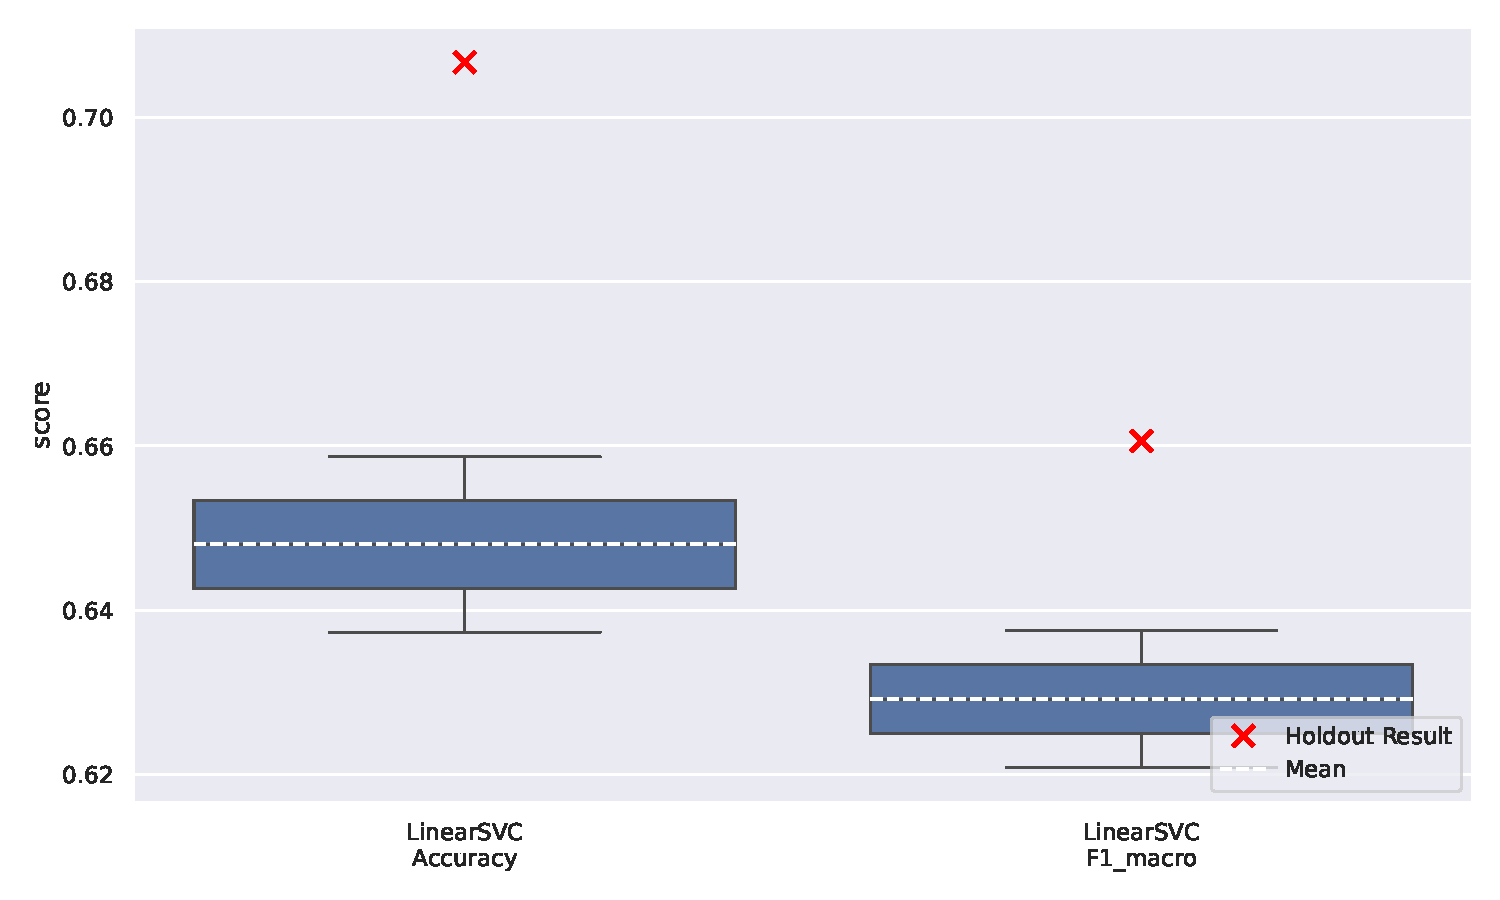
\includegraphics[width=\textwidth]{amazon/plots/model_comparison.pdf}
\caption{Model Comparison for \textit{'Amazon Commerce Reviews'} dataset}
\label{fig:model_comparison amazon}
\end{figure}





In contrast, for the dataset 
\textit{'Census Income'} the hold-out scores are almost the same as the mean of the cross-validation, which is to be
expected because this dataset has a lot of instances. The box-plots for this dataset (figure 9) are also
comparatively very narrow, meaning that the scores calculated during cross-validation vary very little i.e.
the variance is really low.




We also want compare the efficiency of the classifiers. For this we used the runtime of the hold-out
method calculation from above. We measured both the time for training (including preprocessing) and
the time it took the test the model. Those values are displayed in table~\ref{tab:runtime_models}.


\begin{table}[h!]
\centering
\footnotesize
\begin{tabular}{|c|c|c|c|c|c|c|c|c|}
\hline
\textbf{Model} & \multicolumn{2}{c|}{Census} & \multicolumn{2}{c|}{Amazon} & \multicolumn{2}{c|}{Congress} & \multicolumn{2}{c|}{Diabetes} \\
\hline
& \textbf{Train} & \textbf{Pred} & \textbf{Train} & \textbf{Pred} & \textbf{Train} & \textbf{Pred} & \textbf{Train} & \textbf{Pred} \\
\hline
LinearSVC & 0.17 & 0.02 & 0.51 & 0.02 & 0.00 & 0.00 & 0.00 & 0.00 \\
\hline
Ridge & 0.09 & 0.02 & 7.91 & 0.20 & 0.00 & 0.00 & 0.00 & 0.00 \\
\hline
RandomForest & 126.59 & 1.63 & 12.92 & 0.10 & 1.00 & 0.03 & 4.79 & 0.09 \\
\hline
\end{tabular}
\vspace{0.3cm}
\caption{Runtime of models for different datasets}
\label{tab:runtime_models}
\end{table}




On the contrary, the linear support vector classifier and ridge classifier performed similar
on the first glance. The results from \textit{'Amazon Commerce Reviews'} and \textit{'Census Income'} might suggest,
that the linear support vector classifier is faster for high dimensional datasets, whereas the ridge classifier
is quicker with a high number of instances. We found out that the parameter dual of the linear support
vector classifier has a great influence on its runtime. This parameter describes whether the algorithm
should solve for the primal or dual optimization problem. Let n be number of samples and d the number
of dimensions of a dataset. The dual formulation requires the computation of a n × n matrix, whereas
in the primal formulation a d × d matrix is calculated. Therefore the primal formulation is faster for
datasets, where n > d, which was especially noticeable for the ”Census Income” dataset. Also on the~\textit{'Diabetes'}
dataset as it is very low dimensional the dual prosedure is faster. The results are shown in table~\ref{tab:dual_comparison}.

\begin{table}[h!]
\centering
\begin{tabular}{|c|c|c|}
\hline
\textbf{Dataset} & \textbf{Normal} & \textbf{Dual} \\
\hline
Census & 0.198 & 1.43 \\
\hline
Amazon & 2.27 & 0.648 \\
\hline
Census & 0.005 & 0.007 \\
\hline
Diabetes & 0.004 & 1.25 \\
\hline
\end{tabular}
\vspace{0.3cm}
\caption{Comparison of Dual and Normal Ridge classifier training time for different datasets}
\label{tab:dual_comparison}
\end{table}
After all experiments our final conclusion is that no classifier we used outperformed the other across all
datasets. The results in table \ref{tab:best_results} imply that the effectiveness of a classifier is highly dependent on the
dataset. What we can establish is that the linear support vector classifier was never the worst in both
metrics. Therefore it seems to be a very versatile classifier. In comparison the success for random forests
varied quite a lot for different datasets and effectiveness measures. This could be due to the fact, that
decision trees generally tend to overfit the model. As for efficiency, table \ref{tab:runtime_models} highlighted a big weakness of
the random forest classifier, namely that it’s comparatively very slow. Summing up section \ref{preprocessing}, choosing
the right preprocessing steps, especially the scaler and dimension reduction, influences the results notably,
though in varying magnitude for different classifiers and datasets. Here random forest seems the be the
least influenced by the choice of scaler as seen in tables \ref{table:censustransformers} and \ref{table:diabetesscalers}. The sensitivity analysis in section \ref{einfügen}
showed how much of an impact even a single hyperparameter can have on the overall performance of a
model. However, comparing the results of section \ref{sec:preprocessing} with the ones in section \ref{sec:hyperparameters} and table \ref{tab:runtime_models}, it is clear that
tuning the parameters hardly influenced the result for the ”congressional voting” dataset. In contrast, the
recall score for the ”diabetes” dataset and both effectiveness scores for the ”Amazon Commerce Reviews”
improved a lot after the parameter tuning. For the dataset ”Census Income” only the support vector
classifier improved after optimizing the F1 score. As a summary of this whole project we would say that
the best strategy for a classification problem majorly depends on the dataset in the beginning. Once a
classifier is chosen everything else depends on the combination of the two including the importance of
parameter tuning and preprocessing as well as the overall success.




\end{document}